% \documentclass[twocolumn]{article}
%\documentclass[10pt,conference]{IEEEtran}
\RequirePackage{rotating}
\documentclass[sigconf]{acmart}
%\documentclass[runningheads]{llncs}

\usepackage{babel}
\usepackage{inputenc}
\usepackage{pifont}
\usepackage[T1]{fontenc}
%\usepackage{lmodern}

%% Math
\usepackage{mathtools}
%%\usepackage{amsmath}
%\usepackage{commath}

\usepackage{amsfonts}% revise se precisa ou não
%\usepackage{nccmath}% revise se precisa ou não

%\usepackage[numbers]{natbib}
\usepackage{multirow}
\usepackage{makecell}
%%\usepackage{graphicx}

\usepackage{listings}
\usepackage{float}
\usepackage{enumitem}

%\usepackage{wasysym}
%\usepackage{resizegather}
\usepackage{rotating}

%\usepackage{caption}
%\captionsetup[table]{skip=5pt}
%\captionsetup[table]{position=above}

\renewcommand{\lstlistingname}{Código}
\renewcommand{\lstlistlistingname}{Lista de \lstlistingname s}

%\definecolor{codegreen}{rgb}{0,0.6,0}
%\definecolor{codegray}{rgb}{0.85,0.85,0.85}
%\definecolor{codepurple}{rgb}{0.58,0,0.82}
%\definecolor{codeblack}{rgb}{0,0,0}

\lstdefinelanguage{JavaScript}{
  keywords={typeof, new, true, false, catch, function, return, null, catch, switch, var, if, in, while, do, else, case, break},
  %keywordstyle=\color{blue}\bfseries,
  ndkeywords={class, export, boolean, throw, implements, import, this},
  %ndkeywordstyle=\color{codegray}\bfseries,
  %identifierstyle=\color{black},
  sensitive=false,
  comment=[l]{//},
  morecomment=[s]{/*}{*/},
  %commentstyle=\color{purple}\ttfamily,
  %stringstyle=\color{red}\ttfamily,
  morestring=[b]',
  morestring=[b]"
}

\lstdefinestyle{codigo}{
    backgroundcolor=\color{codegray},   
    commentstyle=\color{codegreen},
    keywordstyle=\color{magenta},
    numberstyle=\tiny\color{codeblack},
    stringstyle=\color{codepurple},
    basicstyle=\ttfamily\footnotesize,
    breakatwhitespace=false,         
    breaklines=true,                 
    captionpos=b,                    
    keepspaces=true,                 
    numbers=left,                    
    numbersep=5pt,                  
    showspaces=false,                
    showstringspaces=false,
    showtabs=false,                  
    tabsize=4
}

\lstset{style=codigo}

\DeclarePairedDelimiter{\round}\lfloor\rceil
\newcommand\citetxt[1]{%
  \citeauthor{#1}~(\citeyear{#1})}
\newcommand\citepar[1]{%
  (\citeauthor{#1}, \citeyear{#1})} 
  


%https://tex.stackexchange.com/q/151984/7561
\DeclarePairedDelimiterX{\infdivx}[2]{(}{)}{%
  #1\;\delimsize\|\;#2%
}
\newcommand{\kl}{\operatorname{KL}\infdivx}
\newcommand{\skl}{\operatorname{SKL}\infdivx}

% https://tex.stackexchange.com/questions/23773/a-centered-plus-minus-symbol
\newcommand{\rpm}{\raisebox{.2ex}{$\scriptstyle\pm$}}

% https://tex.stackexchange.com/a/141685/7561
\newcommand\givenbase[1][]{\:#1\lvert\:}
\let\given\givenbase

% https://tex.stackexchange.com/a/171959/7561
\newcommand\reallywidehat[1]{\ThisStyle{%
    \setbox0=\hbox{$\SavedStyle#1$}%
    \stackengine{-1.0\ht0+.5pt}{$\SavedStyle#1$}{%
      \stretchto{\scaleto{\SavedStyle\mkern.15mu\char'136}{1.5\wd0}}{1.4\ht0}%
    }{O}{c}{F}{T}{S}%
}}
\newcommand{\hkl}{\widehat{\operatorname{KL}}\infdivx}

% Conditional independence symbol
% https://tex.stackexchange.com/questions/218631/symbol-for-not-conditionally-independent/
\newcommand{\CI}{\mathrel{\perp\mspace{-10mu}\perp}}

% declare my argmin and argmax operators
% https://tex.stackexchange.com/a/5255/7561
\DeclareMathOperator*{\argmax}{arg\,max}
\DeclareMathOperator*{\argmin}{arg\,min}

% declaring an expectation operator to behave like sum
% https://tex.stackexchange.com/a/23436/7561
\makeatletter
\DeclareRobustCommand\bigop[1]{%
  \mathop{\vphantom{\sum}\mathpalette\bigop@{#1}}\slimits@
}
\newcommand{\bigop@}[2]{%
  \vcenter{%
    \sbox\z@{$#1\sum$}%
    \hbox{\resizebox{\ifx#1\displaystyle.9\fi\dimexpr\ht\z@+\dp\z@}{!}{$\m@th#2$}}%
  }%
}
\makeatother

% Keywords command
\providecommand{\keywords}[1]
{
  \small	
  \textbf{\textit{Keywords ---}} #1
}
\providecommand{\palavraschave}[1]
{
  \small	
  \textbf{\textit{Palavras-chave ---}} #1
}

%\newcommand{\E}{\DOTSB\bigop{\mathbb{E}}}
\DeclareMathOperator*{\E}{\mathbb{E}}

% redefining \times operator
\let\oldtimes\times
\def\times{{\mkern1mu\oldtimes\mkern1mu}}



\usepackage{subfigure}
\newcommand{\cmark}{\ding{51}}%

%\DeclarePairedDelimiter\abs{\lvert}{\rvert}%
%\DeclarePairedDelimiter\norm{\lVert}{\rVert}%
\DeclarePairedDelimiter\product{\langle}{\rangle}%

%\usepackage{cellspace}
%\setlength\cellspacetoplimit{6pt}
%\setlength\cellspacebottomlimit{4pt}

%% Units
\usepackage{siunitx}

%% Tables
\usepackage{booktabs}

\usepackage{comment}


% Para acrescentar comentários ao PDF descomente:
\usepackage
%  [pdfauthor={nome do autor},
%   pdftitle={titulo},
%   pdfkeywords={palavra-chave, palavra-chave},
%   pdfproducer={Latex with hyperref},
%   pdfcreator={pdflatex}]
{hyperref}

% Os cores podem ser mudados
\hypersetup{
%  linkcolor={red!50!black},
%  citecolor={blue!50!black},
%  urlcolor={blue!80!black}
}

\usepackage{url}
\usepackage{breakurl}
% \usepackage[breaklinks]{hyperref}

\def\UrlBreaks{\do\/\do-\do\_}

\title{A semi-autonomic framework for developing Machine Learning-based applications using Fairness metrics}
\begin{comment}
\author{Thales Eduardo Nazatto}
\email{tenazatto@gmail.com}
\affiliation{%
  \institution{University of Campinas}
  \streetaddress{P.O. Box 1212}
  \city{Campinas}
  \state{São Paulo}
  \country{Brazil}
  \postcode{43017-6221}
}

\author{Cecília Mary Fischer Rubira}
\email{cmrubira@ic.unicamp.br}
\affiliation{%
  \institution{University of Campinas}
  \streetaddress{P.O. Box 1212}
  \city{Campinas}
  \state{São Paulo}
  \country{Brazil}
  \postcode{43017-6221}
}

\author{Leonardo Montecchi}
\email{leonardo.montecchi@ntnu.no}
\affiliation{%
  \institution{Norwegian University of Science and Technology}
  \city{Trondheim}
  \state{Trøndelag}
  \country{Norway}
}
\end{comment}

%\settopmatter{printacmref=false}
%\setcopyright{none}
%\renewcommand\footnotetextcopyrightpermission[1]{}
\setcopyright{acmcopyright} % if you give the rights to ACM
\acmDOI{xx.xxx/xxx_x} % DOI - Insert your DOI below...
\acmISBN{979-8-4007-0243-3/24/04} % ISBN - Insert your conference/workshop's ISBN below...
\acmYear{2024} % Insert Publication year
\copyrightyear{2024} % Insert Copyright year (typically the same as above)
\acmArticle{4}
\acmPrice{15.00}
\acmConference[SAC'24]{ACM SAC Conference}{April 8-12 2024}{Avila, Spain}

\hyphenation{ex-ten-si-bil-i-ty}
\hyphenation{com-put-ing}
\hyphenation{soft-ware}
\hyphenation{re-spon-si-bil-i-ty}
\hyphenation{Mon-tec-chi}
\hyphenation{ob-jec-tives}
\hyphenation{au-tomat-ing}
\hyphenation{en-gi-neer-ing}
\hyphenation{au-to-mate}
\hyphenation{au-to-mat-ed}
\hyphenation{reweigh-ing}
\hyphenation{re-mover}
\hyphenation{ob-tain-ing}
\hyphenation{ex-po-nen-ti-at-ed}
\hyphenation{im-ple-ment-ed}
\hyphenation{dis-cussed}
\hyphenation{ques-tion-naire}
\hyphenation{clas-si-fi-ca-tion}
\hyphenation{op-ti-mized}
\hyphenation{prob-lems}
\hyphenation{im-ple-men-ta-tion}
\hyphenation{op-por-tu-ni-ty}
\hyphenation{cor-re-spond-ing}
\hyphenation{al-go-rithms}
\hyphenation{be-comes}
\hyphenation{con-tain-ing}
\hyphenation{ex-e-cu-tions}
\hyphenation{met-rics}
\hyphenation{nec-es-sary}
\hyphenation{re-duc-tion}
\hyphenation{au-to-nom-ic}
\hyphenation{pro-posed}
\hyphenation{con-fig-u-ra-tion}
\hyphenation{train-ing}
\hyphenation{dif-fer-ent}
\hyphenation{dif-fer-ence}
\hyphenation{de-vel-op-ers}
\hyphenation{ex-pect-ed}
\hyphenation{mod-i-fi-ca-tion}
\hyphenation{ac-com-mo-date}
\hyphenation{sig-nif-i-cant-ly}
\hyphenation{eval-u-a-tion}
\hyphenation{ar-chi-tec-tur-al}
\hyphenation{aug-men-ta-tion}
\hyphenation{meta-da-ta}
\hyphenation{pro-por-tion-al}
\hyphenation{pro-grammed}
\hyphenation{in-ter-change-able}
\hyphenation{pos-si-bil-i-ties}
\hyphenation{ad-di-tion-al-ly}
\hyphenation{knowl-edge}
\hyphenation{se-quence}
\hyphenation{di-vi-sion}
\hyphenation{pa-ra-me-ter-i-za-tion}

\begin{document}

%IEEETran \maketitle

\begin{abstract}
The increasing use of Machine Learning (ML) in digital solutions has created a need for new algorithms and fairness metrics to ensure fairer decisions. However, this has made data scientist analysis more complex, due to the need to balance fairness metrics with traditional evaluation metrics and a greater variety of algorithms. This work presents a semi-autonomous framework to train machine learning models that identifies more optimized configurations across different contexts. The framework uses a module using the \textit{Pipes-and-Filters} architecture with several pre-implemented algorithms and a module using the MAPE-K architecture to evaluate the ideal balance. Several case studies were conducted to determine the feasibility and extensibility of the proposed framework. The results showed that the framework can help data scientists better understand the training process and enable software engineering studies to help train trustworthy machine learning models.
\end{abstract}

\begin{CCSXML}
<ccs2012>
<concept>
<concept_id>10010147.10010257</concept_id>
<concept_desc>Computing methodologies~Machine learning</concept_desc>
<concept_significance>500</concept_significance>
</concept>
<concept>
<concept_id>10010520.10010521.10010542.10010548</concept_id>
<concept_desc>Computer systems organization~Self-organizing autonomic computing</concept_desc>
<concept_significance>500</concept_significance>
</concept>
<concept>
<concept_id>10010520.10010521.10010522.10010526</concept_id>
<concept_desc>Computer systems organization~Pipeline computing</concept_desc>
<concept_significance>300</concept_significance>
</concept>
<concept>
<concept_id>10010520.10010575.10010579</concept_id>
<concept_desc>Computer systems organization~Maintainability and maintenance</concept_desc>
<concept_significance>100</concept_significance>
</concept>
<concept>
<concept_id>10011007.10011074.10011092.10011096.10011097</concept_id>
<concept_desc>Software and its engineering~Software product lines</concept_desc>
<concept_significance>300</concept_significance>
</concept>
<concept>
<concept_id>10011007.10011074.10011111.10011113</concept_id>
<concept_desc>Software and its engineering~Software evolution</concept_desc>
<concept_significance>100</concept_significance>
</concept>
</ccs2012>
\end{CCSXML}

\ccsdesc[500]{Computing methodologies~Machine learning}
\ccsdesc[500]{Computer systems organization~Self-organizing autonomic computing}
\ccsdesc[300]{Computer systems organization~Pipeline computing}
\ccsdesc[100]{Computer systems organization~Maintainability and maintenance}
\ccsdesc[300]{Software and its engineering~Software product lines}
\ccsdesc[100]{Software and its engineering~Software evolution}

\keywords{Machine Learning, Artificial Intelligence Ethics, Social Responsibility in Artificial Intelligence, Autonomic Computing, Fairness Metrics}

\maketitle
%\pagestyle{plain}

\section{Introduction}

Artificial intelligence (AI) and machine learning (ML) techniques have been used for many years in computer science, particularly in areas such as robotics and games, where they can automate tasks and generate insights from large volumes of data. However, these applications can also introduce biases that reflect existing prejudices in today's society. Biased data entries result in an algorithm that performs discriminations in its classification~\citep{Buolamwini_2018}, and evaluation metrics typically evaluate the entire dataset rather than specific groups, so it can be difficult to detect bias in the results.

Due to this problem, it is possible to establish different metrics to determine how well the model is prepared for sensitive data~\citep{Begley_2021}, a term that is known as Fairness. The main goal of Fairness is to ensure that privileged and non-privileged groups, regardless of their protected attributes, are treated equally, as evidenced by similar metrics. Advances in academic research on fairness have led to new methods for reducing biases present in datasets, such as \textit{Reweighing}~\citep{Kamiran_2011}, \textit{Adversarial Debiasing}~\citep{Zhang_2018} and \textit {Reject Option Classification}~\citep{Kamiran_2012}. While these methods have improved fairness metrics, they may disfavor other metrics that are widely used to assess the effectiveness of machine learning models.

For this context, a framework for developing Machine Learning applications was developed~\footnote{Repository containing the code implementation: \url{https://anonymous.4open.science/r/FAIR-2EFD}}, which is handled by Data Scientists in a semi-autonomous way, focused on two main objectives:

\begin{itemize}
\item Facilitate the creation of fair and reliable models by automating the following process: Data preparation, training and evaluation.
\item Establish a balance between Evaluation metrics and Fairness metrics to efficiently obtain fairer models.
\end{itemize}

\begin{figure*}[h]
\centering
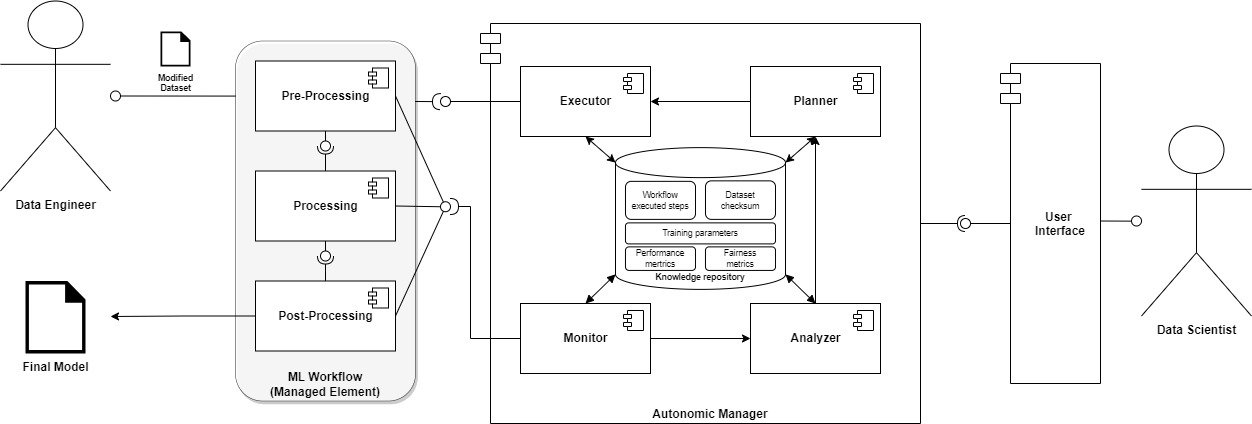
\includegraphics[scale=0.285]{images/backend-frontend-ml-eng.jpg}
\caption {Architecture components of the proposed framework}
\label{fig:BackendFrontendML}
\end{figure*}

This structure is divided into 4 modules: Data Engineering, ML Module, Autonomic Manager, and User Interface. The Data Engineering module prepares the data for the ML Module by modifying the German Credit Dataset~\citep{ucigerman_2021} and Lendingclub Dataset~\citep{lendingclub_2022} datasets. The ML Module is developed using the \textit{Pipes-and-Filters} architecture. For the Autonomic Manager, the MAPE-K~\citep{IBM_2005} architecture analyzes a knowledge repository to identify the best architectural configuration for the ML Module. The User Interface is a web application template.

\section{The Proposed Framework}

\subsection{Architecture and Implementation}

%\begin{figure*}[h]
%\centering
%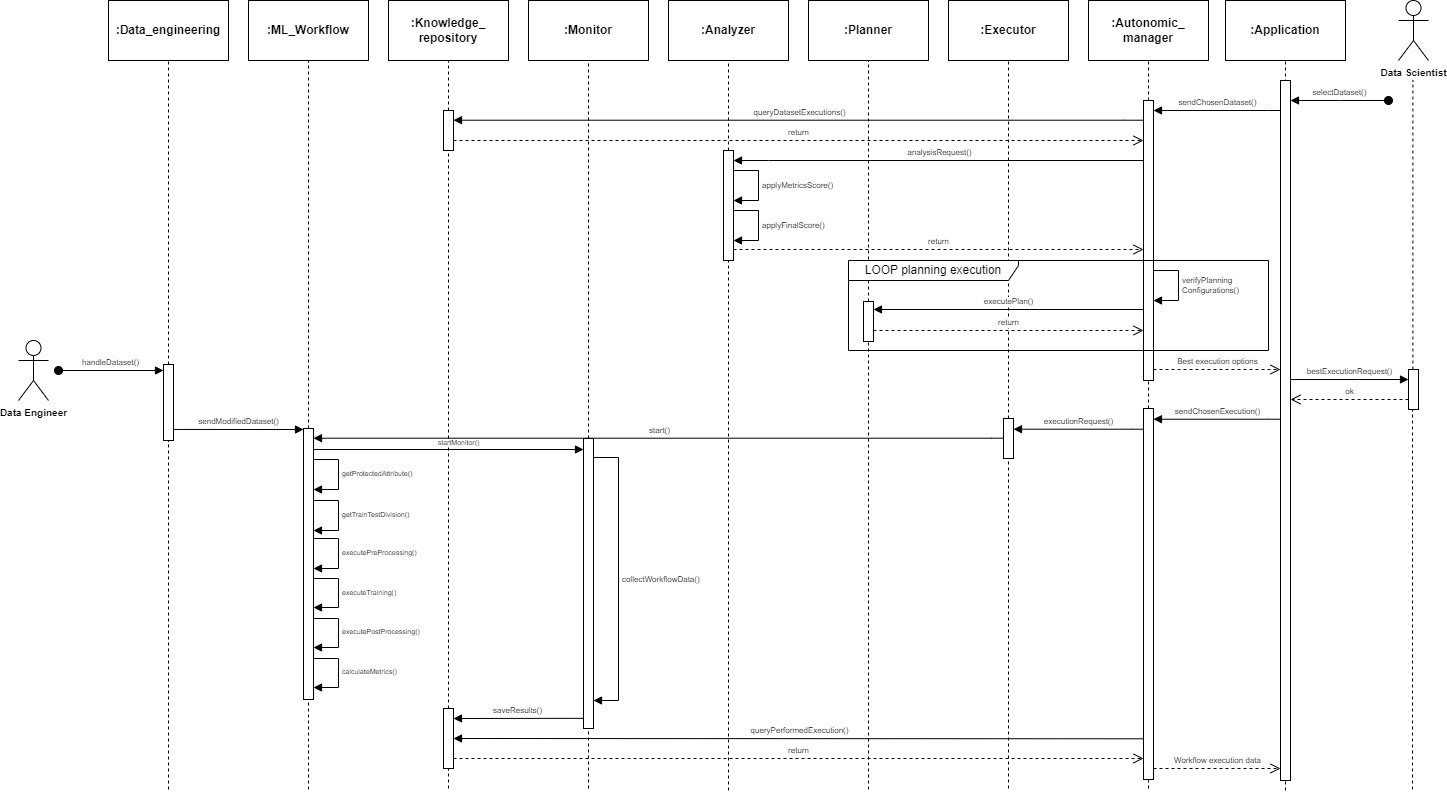
\includegraphics[scale=0.35]{images/Diagrama_Sequencia-eng.jpg}
%\caption {System's sequence diagram}
%\label{fig:DiagramaSequencia}
%\end{figure*}
\begin{sidewaysfigure*}
\clearpage
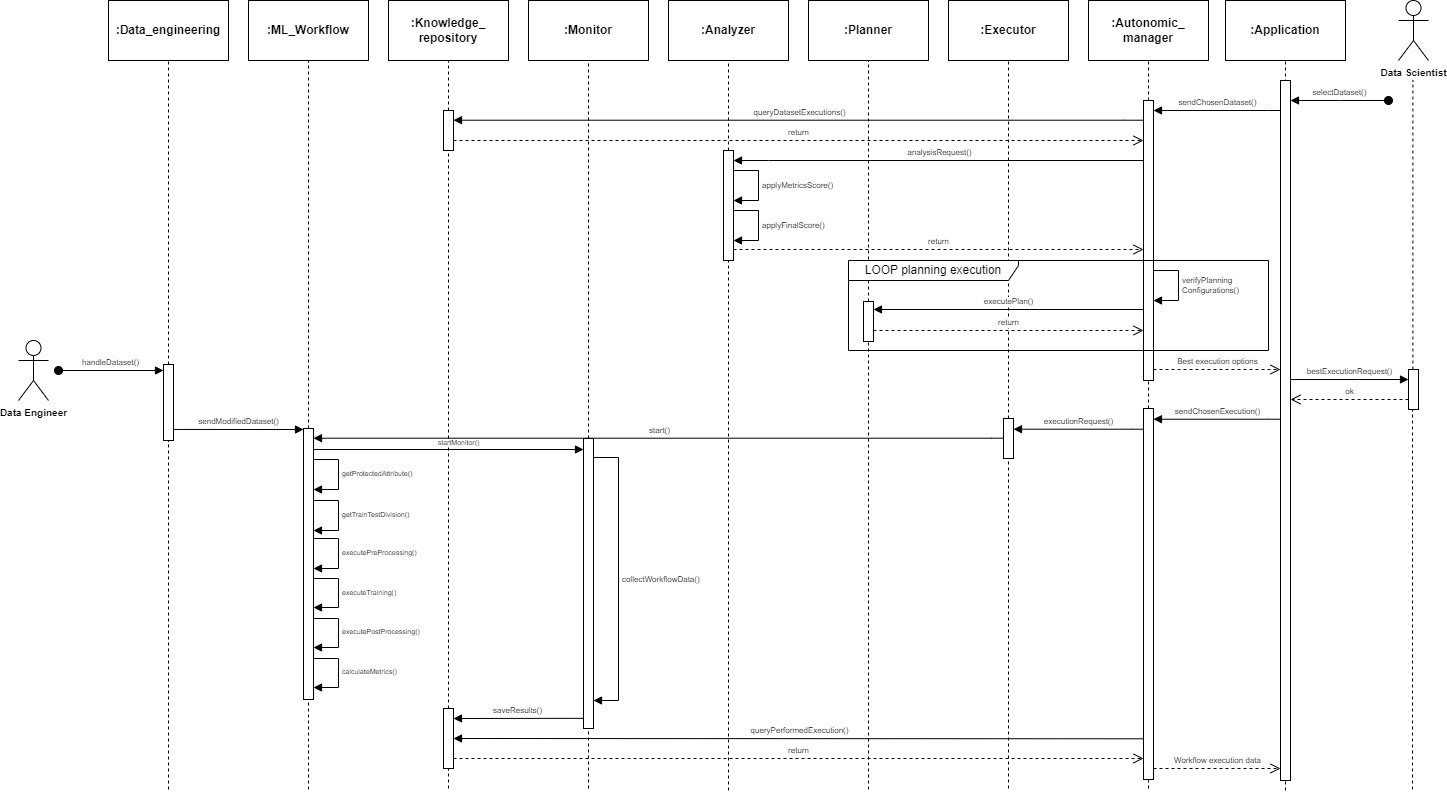
\includegraphics[scale=0.395]{images/Diagrama_Sequencia-eng.jpg}
\caption {Sequence diagram with help of the Autonomic Manager}
\label{fig:DiagramaSequencia}
\end{sidewaysfigure*}

The framework architecture is divided into 4 modules:

\begin{itemize}
    \item {\textbf{Data Engineering:}} Module with the objective of executing data transformation and cleaning processes.
	\item {\textbf{ML Module:}} Module that executes a Pipeline of an automated ML application, with stages of data preparation (Pre-pro\-cess\-ing), training (Processing) and result evaluation (Post-processing) of the final model generation.
     \item {\textbf{Autonomic Manager:}} Module containing a MAPE-K control \textit{loop} that controls the ML Module as a Managed Element to automate all its steps.
     \item {\textbf{User Interface):}} Module which goal is to provide a simpler and more intuitive user experience for the Data Scientist in order to configure and start the Autonomic Manager.
\end{itemize}

The integration between these modules is illustrated in Figure \ref{fig:BackendFrontendML}. The Data Engineering module is used by the Data Engineer to prepare the dataset for execution in the ML Module. The User Interface module is used by the Data Scientist to specify the architectural configuration, which depends on the context of the problem. The ML Module can be executed manually or with the help of the Autonomic Manager.

The process of manual execution can be visualized in the Sequence Diagram in Figure \ref{fig:DiagramaSequenciaModuloML}. The Data Engineer first prepares the dataset using the Data Engineering module and stores them in the knowledge repository. The Data Scientist then starts the ML Module, passing in the necessary parameters. During execution, the ML Module starts the Monitor component from Autonomic Manager to collect data during execution, retrieves the dataset from the knowledge repository and executes the preprocessing, processing, and post-processing steps defined by the passed parameters to generate the final model. At the end of the execution, the Monitor saves all collected data in the knowledge repository for future use.

\begin{figure*}[h]
\centering
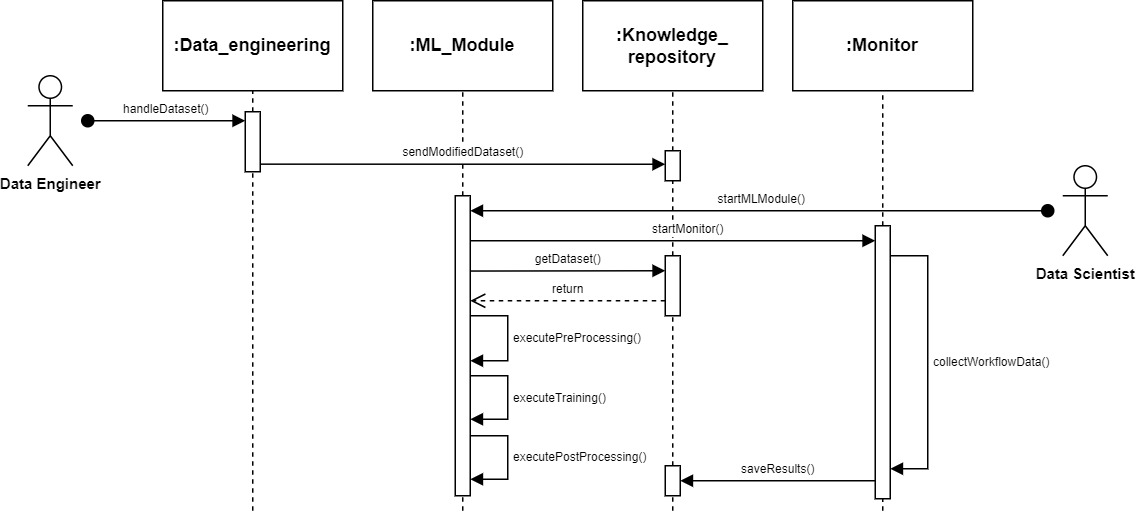
\includegraphics[scale=0.425]{images/Diagrama_Sequencia-manual-eng.jpg}
\caption{Sequence diagram from a manual ML Module execution}
\label{fig:DiagramaSequenciaModuloML}
\end{figure*}

The process of execution with the help of the Autonomic Manager can be visualized in the Sequence Diagram in Figure \ref{fig:DiagramaSequencia}. The Data Scientist, through the User Interface module, selects the dataset and requests an execution. The Autonomic Manager then searches for all previous executions of the ML Module that have already used the modified dataset and are stored in the knowledge repository. It then performs an analysis by performing calculations presented in section~\ref{sec:AnalyzerComponent}. Next, the Autonomic Manager then loops through the configuration of existing execution plans and executes them. It then returns the best execution options to the Data Scientist, who can choose the most appropriate option and request a new execution for the ML Module. This execution is equivalent to the one already explained in Figure \ref{fig:DiagramaSequenciaModuloML}. The Autonomic Manager then searches for the data from this execution to display it to the Data Scientist in the Interface.

\subsection{The ML Module}

The ML module is parameterized to allow the Data Scientist to control the architectural configuration used in its execution. This includes the dataset, protected attribute, and algorithms used. It is implemented using the \textit{Pipes-and-Filters} architecture, which allows for interchangeable Pipes and Filters depending on the parameterization used, making it easy to program execution plans within the Autonomic Manager. These Pipes and Filters are divided into three types of components, illustrated in Figure \ref{fig:BackendFrontendML}, categorized by the newly developed algorithms that were created to improve the learning process's ability to handle biased data: 

\begin{itemize}
\item \textbf{Pre-processing:} These algorithms try to remove biased data by transforming it. The implemented algorithms in these components are \textit{Disparate Impact Remover}~\citep{Feldman_2015}, \textit{Learning Fair Representations}~\citep{Zemel_2013}, \textit{Reweighing}~\citep{Kamiran_2011} and \textit{Optimized Preprocessing}~\citep{Calmon_2017}.
\item \textbf{Processing:} These algorithms try to mitigate discrimination during the training process. The implemented algorithms in these components are \textit{Adversarial Debiasing}~\citep{Zhang_2018}, \textit{Exponentiated Gradient Reduction}~\citep{Agarwal_2018}, \textit{Grid Search Reduction}~\citep{Agarwal_2019}, \textit{Meta Fair Classifier}~\citep{Celis_2019}, \textit{Prejudice Remover}~\citep{Kamishima_2012} and \textit{Rich Subgroup Fairness}~\citep{Kearns_2018}.
\item \textbf{Post-processing:} These algorithms modify the predictions of an already trained model to produce fairer outcomes. The implemented algorithms in these components are \textit{Equalized Odds}~\citep{Hardt_2016}, \textit{Calibrated Equalized Odds}~\citep{Pleiss_2017} and \textit{Reject Option Classification}~\citep{Kamiran_2012}.
\end{itemize}

Some steps were additionally implemented in the Pre-processing components: The acquisition of the dataset; acquisition of the protected attribute, privileged group, and unprivileged group; division of the dataset into train, validation and test sets; the data preparation based in the protected attribute, privileged group, and unprivileged group. Because Pre-processing and Post-processing algorithms are not part of model training, Logistic Regression, Gradient Boosting, Random Forest and Support Vector Machines were additionally implemented in the Processing components. The calculation of Evaluation and Fairness metrics was additionally implemented in the Post-processing components.

\subsection{Monitor Component}

The Monitor is initiated along with the execution of the ML Module, as illustrated in Figure \ref{fig:DiagramaSequenciaModuloML}. The following metadata are stored:

\begin{itemize}
\item \textbf{Pre-processing}: Parameters related to the architectural configuration executed by the module (dataset, protected attribute, and pre-processing algorithm) and the checksum of the dataset used.
\item \textbf{Processing}: Parameters related to the architectural configuration executed (training algorithm) and parameters used for training.
\item \textbf{Post-processing}: Parameters related to the architectural configuration executed (post-processing algorithm) and metrics of the resulting model (evaluation metrics and fairness metrics).
\end{itemize}

The data collected per execution are organized into two different sets: One containing the metadata and information related to the architectural configuration executed by the ML Module, and one containing the metrics obtained by the resulting model from that execution. Both sets have an execution identifier to establish consistency between the data in the two sets. This organization facilitates the development of the Analyzer component.

\subsection{Analyzer Component}
\label{sec:AnalyzerComponent}

The Analyzer extracts and analyzes ML Module executions from the knowledge repository based on their metrics, assigning each execution a score that consolidates its evaluation and fairness metrics. The analyses are then grouped by architectural configuration, and each configuration receives a final score. The scores for each architectural configuration are grouped together and placed in a dataset, with additional metadata such as execution date. This dataset is then passed to the Planner to help develop better strategies.

\begin{figure}[h]
\centering
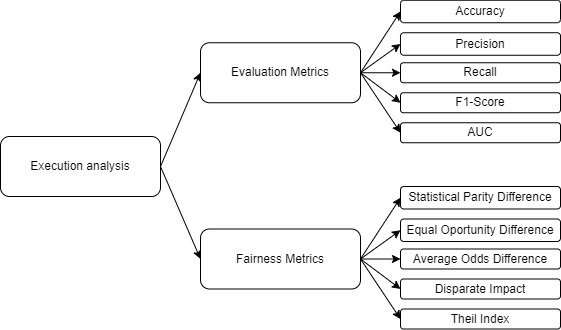
\includegraphics[scale=0.425]{images/metrics-tree.jpg}
\caption {Metrics tree used in execution analysis}
\label{fig:MetricTree}
\end{figure}

To analyze each execution made by the ML Module, the metrics are weighted according to their importance in the context of the problem, as determined by the Data Scientist. This is done to consolidate the evaluation and fairness metrics into a single score, which simplifies planning strategies. This calculation uses a metrics tree, illustrated in Figure \ref{fig:MetricTree}, to divide the metrics into two groups: Evaluation Metrics and Fairness Metrics. The Evaluation Metrics group includes the metrics Accuracy, Precision, Recall, F1-Score, and Area Under the ROC Curve (AUC). The Fairness Metrics group includes the metrics Statistical Parity Difference, or discrimination~\citep{Zemel_2013}, Equal Opportunity Difference~\citep{Biswas_2020}, Average Odds Difference~\citep{Biswas_2020}, Disparate Impact~\citep{Biswas_2020} and Theil Index~\citep{Speicher_2018}. The weights $w_E$ for the Evaluation Metrics group and $w_F$ for the Fairness Metrics group are assigned and the way used to consolidate all metrics was through a score $S$ defined by a weighted mean, displayed in equation \ref{eqn:totalScore}, between the $S_E$ and $S_F$ scores.

\begin{equation}
\label{eqn:totalScore}
	S = \frac{w_F \times S_F + w_E \times S_E}{w_F + w_E}
\end{equation}

To calculate the $S_E$ and $S_F$ for the Evaluation Metrics and Fairness Metrics groups, respectively, a weighted mean is calculated for each group. The weights for each metric are denoted by $w_{m_{Ei}}$ for the Evaluation Metrics group and $w_{m_{Fi}}$ for the Fairness Metrics group, but there are some differences to consider given the nature of the metrics in each group In the case of $S_E$, all calculated metrics are in the interval $\left[0,1 \right]$ and their results are directly proportional, meaning that the best results have the highest values. This implies that a weighted mean can be used without any modifications.

\begin{equation}
\label{eqn:EvaluationScore}
	\begin{aligned}
	S_{E} = \frac{\sum_{i=1}^{n_{m_E}} w_{m_{E_i}} \times m_{E_{i}}}{\sum_{i=1}^{n_{m_E}} w_{m_{E_i}}}
	\end{aligned}
\end{equation}

In the equation \ref{eqn:EvaluationScore}, $n_{m_E}$ is the number of evaluation metrics used (for the tree defined in Figure \ref{fig:MetricTree}, $n_{m_E} = 5$), $w_{m_{E_i}}$ is the weight given to a given evaluation metric and $m_{E_{i}}$ is the value of a given evaluation metric in the analyzed execution.

However, for the case of $S_F$, there are three different intervals and situations for the Fairness metrics present in the group:

\begin{itemize}
	\item \textbf{Statistical Parity Difference}, \textbf{Equal Opportunity Difference} and \textbf{Average Odds Difference} involve the difference between two or more indicators in the interval $\left[0,1 \right]$, being in the interval $\left[-1,1 \right]$ and 0 is considered the best result.
	\item \textbf{Theil Index} is in the interval $\left[0,1 \right]$, but it is inversely proportional: 0 is considered the best result and 1 the worst.
	\item \textbf{Disparate Impact} is the only that involves the ratio of two indicators, being in the interval $\left[0,+\infty \right[$ and 1 is considered the best result.
\end{itemize}

To normalize the fairness metrics $m_{F_i}$ to a metric $m'_{F_i}$ in the interval $\left[0,1 \right]$, each case was treated separately. For the first two cases, $m'_{F_i} = 1-\lvert m_{F_i} \rvert$ is used because produces the same results. For the third case, it needed another calculation. The following equation consolidates all cases:

\begin{equation}
\label{eqn:normalizationFairnessStep3}
	\begin{aligned}
	m'_{F_i} = 
	\begin{cases}
	1-\lvert \frac{1}{m_{F_i}}-1 \lvert & \text{if $m_{F_i}$ is Disparate Impact e $m_{F_i} > 1$}\\
	1-\lvert m_{F_i}-1 \lvert & \resizebox{0.56\hsize}{!}{\text{if $m_{F_i}$ is Disparate Impact and $0 \leqslant m_{F_i} \leqslant 1$}}\\
	1-\lvert m_{F_i} \rvert & \text{otherwise}
	\end{cases}
	\end{aligned}
\end{equation}

After obtaining $m'_{F_i}$, it is possible to obtain $S_F$ using another weighted mean:

\begin{equation}
\label{eqn:FairnessScore}
	\begin{aligned}
	S_{F} = \frac{\sum_{i=1}^{n_{m_F}} w_{m_{F}} \times m'_{F_{i}}}{\sum_{i=1}^{n_{m_F}} w_{m_{F_i}}}
	\end{aligned}
\end{equation}

In the equation \ref{eqn:FairnessScore}, $n_{m_F}$ is the number of fairness metrics used (for the tree defined in Figure \ref{fig:MetricTree}, $n_{m_F} = 5$), $w_{m_{F_i}}$ is the weight given to a given fairness metric, and e $m'_{F_{i}}$ is the value of a given fairness metric in the analyzed execution that was normalized to the interval $\left[0,1 \right]$. 

To consolidate the final scores $S'_E$, $S'_F$ e $S'$ for each architectural configuration, each execution is grouped according to the architectural configuration used, and a simple arithmetic mean is calculated according to the $n'$ executions found for that configuration. To facilitate the visualization of the scores in the Interface module by the Data Scientist, the scores $S'_E$, $S'_F$ e $S'$ are multiplied by an arbitrary factor $X = 1000$ and then rounded, as shown in equation \ref{eqn:roundedScore}.

\begin{equation}
\label{eqn:roundedScore}
\resizebox{0.9\hsize}{!}{$
	S'_F = \round*{X \times \frac{\sum_{i=1}^{n'} S_{F_i}}{n'}}\;\;\;\;\;
	S'_E = \round*{X \times \frac{\sum_{i=1}^{n'} S_{E_i}}{n'}}\;\;\;\;\;
	S' = \round*{X \times \frac{\sum_{i=1}^{n'} S_i}{n'}}
$}
\end{equation}

\subsection{Planner Component}

To determine the architectural configuration that will be executed, some strategies were implemented in the Planner component:

\begin{itemize}
\item \textbf{Algorithm filtering}: Algorithms that may not perform well on ML Module or whose models have metrics that require further analysis by the Data Scientist are filtered out before selecting the ideal models.
\item \textbf{Result range}: A minimum and maximum score range is used to determine scores that can be considered reliable for evaluation, thus reducing distortions caused by executions with unreliable metric results.
\end{itemize}

After evaluating these strategies, the Planner component will return the best 5 scores for the Data Scientist to choose, and will ask the Executor to run the ML Module again after choosing.

\section{Framework Evaluation}

Three case studies were conducted to assess the feasibility of the framework, future maintenance, and the ability of the Autonomic Manager to select the best options in different contexts. In all cases, the goal was to predict a credit rating (suitable or not suitable) using a fixed set of \textit{features} in a chosen dataset. In the case of system evolutions, the lines of code performed in each change were also counted, to define whether such changes are simple to make.

The best architectural configurations were evaluated with 3 different weightings in the overall score:

\begin{itemize}
\item 50\% for Evaluation metrics and 50\% for Fairness metrics, for a balanced setup.
\item 75\% for Evaluation metrics and 25\% for Fairness metrics, for a configuration that prioritizes quality over fairness.
\item 25\% for Evaluation metrics and 75\% for Fairness metrics, for a configuration that prioritizes fairness over quality.
\end{itemize}

All executions were performed using a knowledge repository containing approximately 650 previous executions with various architectural configurations of datasets, protected attributes, and algorithms. The repository includes all the evaluation and fairness metrics described on section \ref{sec:AnalyzerComponent}, and all of which are weighted equally within their respective groups.

Since no studies were found where bias reduction is used in more than one step of the machine learning process, only one bias reduction algorithm is performed per execution. Due to unreliable data, executions with the algorithms \textit{Optimized Preprocessing} and \textit{Reject Option Classification} were filtered, corresponding to approximately 5\% of total base size.

\subsection{Case Study 1: Autonomic Manager feasibility and usefulness}

This case study evaluated the behavior of the Autonomic Manager using the German Credit Dataset~\citep{ucigerman_2021}. Age and nationality were used as protected attributes, and a result range of 500 to 950. The results are presented in Tables \ref{tbl:ScoreMAPEKOverall5050}, \ref{tbl:ScoreMAPEKOverall7525}, and \ref{tbl:ScoreMAPEKOverall2575}.

Two surprising observations were made in these executions. First, post-processing algorithms were predominantly used, especially in settings that prioritized quality. This is contrary to the expectation that fairness-enhancing algorithms would improve fairness at the expense of quality. Second, pre-processing algorithms combined with Support Vector Machines as the training algorithm were predominant in configurations that prioritized fairness.

In all executions, it was found that it is difficult to identify the most balanced choice between the two groups of metrics due to the large number of metrics and algorithms used. Additionally, the difference between the metrics is very small, making the choice even more difficult. Consolidating the metrics into groups simplifies the visualization of which architectural configurations are more balanced. The use of weights for each metric and each group could be calibrated to achieve the best desired balance for a given situation. 

In a development context, the Autonomic Manager simplifies the Data Scientist's decision-making and significantly reduces the time to obtain and deploy an optimized model. This is because it eliminates the need to execute multiple algorithms due to the availability of a prior knowledge repository. Additionally, there could be processing and cost savings in the event of future problems with the same dataset, as the executions saved by the teams that use this process can be used by other teams to verify better choices.

\begin{table}[H]
\begin{center}
  \caption{Best configurations chosen by Autonomic Manager \\ 50\% Evaluation/50\% Fairness}
\label{tbl:ScoreMAPEKOverall5050}
  \resizebox{\linewidth}{!}{%
\begin{tabular}{c|c|c|c|c|c|c}
\multicolumn{4}{c|}{Architectural Configuration} & \multicolumn{3}{c}{Score} \\
\hline
Protected attribute & Pre-processing & Processing & Post-processing & Evaluation & Fairness & \textbf{Overall} \\
\hline
Age & Nothing & Logistic Regression & Equalized Odds & 968 & 860 & \textbf{914} \\
Nationality & Nothing & Random Forest & Calibrated Equalized Odds & 902 & 922 & \textbf{912} \\
Nationality & Nothing & Gradient Boosting & Calibrated Equalized Odds & 870 & 925 & \textbf{898} \\
Age & Nothing & Gradient Boosting & Equalized Odds & 927 & 862 & \textbf{894} \\
Age & Reweighing & Gradient Boosting & Nothing & 804 & 931 & \textbf{868} \\
\end{tabular}}
\end{center}
\end{table}

\begin{table}[H]
\begin{center}
  \caption{Best configurations chosen by Autonomic Manager \\ 75\% Evaluation/25\% Fairness}
\label{tbl:ScoreMAPEKOverall7525}
  \resizebox{\linewidth}{!}{%
\begin{tabular}{c|c|c|c|c|c|c}
\multicolumn{4}{c|}{Architectural Configuration} & \multicolumn{3}{c}{Score} \\
\hline
Protected attribute & Pre-processing & Processing & Post-processing & Evaluation & Fairness & \textbf{Overall} \\
\hline
Age & Nothing & Logistic Regression & Equalized Odds & 968 & 860 & \textbf{941} \\
Age & Nothing & Gradient Boosting & Equalized Odds & 927 & 862 & \textbf{910} \\
Nationality & Nothing & Random Forest & Calibrated Equalized Odds & 902 & 922 & \textbf{907} \\
Nationality & Nothing & Gradient Boosting & Calibrated Equalized Odds & 870 & 925 & \textbf{883} \\
Age & Nothing & Random Forest & Equalized Odds & 898 & 799 & \textbf{874} \\
\end{tabular}}
\end{center}
\end{table}

\begin{table}[H]
\begin{center}
  \caption{Best configurations chosen by Autonomic Manager \\ 25\% Evaluation/75\% Fairness}
\label{tbl:ScoreMAPEKOverall2575}
  \resizebox{\linewidth}{!}{%
\begin{tabular}{c|c|c|c|c|c|c}
\multicolumn{4}{c|}{Architectural Configuration} & \multicolumn{3}{c}{Score} \\
\hline
Protected attribute & Pre-processing & Processing & Post-processing & Evaluation & Fairness & \textbf{Overall} \\
\hline
Age & Disparate Impact Remover & Support Vector Machines & Nothing & 747 & 989 & \textbf{928} \\
Nationality & Disparate Impact Remover & Support Vector Machines & Nothing & 747 & 989 & \textbf{928} \\
Age & Nothing & Adversarial Debiasing & Nothing & 742 & 979 & \textbf{920} \\
Nationality & Reweighing & Support Vector Machines & Nothing & 755 & 972 & \textbf{918} \\
Nationality & Learning Fair Representations & Support Vector Machines & Nothing & 755 & 972 & \textbf{918} \\
\end{tabular}}
\end{center}
\end{table}

\subsection{Case Study 2: System evolution by adding a new dataset}

This case study evaluated the Autonomic Manager's versatility in different contexts and the simplicity of system maintenance. The Lendingclub Dataset~\citep{lendingclub_2022} was added in ML Module and used as the dataset, with Income as the protected attribute and a result range of 500 to 980. The results are presented in Tables \ref{tbl:ScoreMAPEKLendingclubOverall5050}, \ref{tbl:ScoreMAPEKLendingclubOverall7525}, and \ref{tbl:ScoreMAPEKLendingclubOverall2575}.

\begin{table}[H]
\begin{center}
  \caption{Best configurations chosen by Autonomic Manager \\ 50\% Evaluation/50\% Fairness}
\label{tbl:ScoreMAPEKLendingclubOverall5050}
  \resizebox{\linewidth}{!}{%
\begin{tabular}{c|c|c|c|c|c|c}
\multicolumn{4}{c|}{Architectural Configuration} & \multicolumn{3}{c}{Score} \\
\hline
Protected attribute & Pre-processing & Processing & Post-processing & Evaluation & Fairness & \textbf{Overall} \\
\hline
Income & Learning Fair Representations & Random Forest & Nothing & 991 & 968 & \textbf{979} \\
Income & Nothing & Gradient Boosting & Equalized Odds & 988 & 969 & \textbf{978} \\
Income & Reweighing & Random Forest & Nothing & 991 & 963 & \textbf{977} \\
Income & Learning Fair Representations & Logistic Regression & Nothing & 981 & 973 & \textbf{977} \\
Income & Reweighing & Gradient Boosting & Nothing & 987 & 964 & \textbf{976} \\
\end{tabular}}
\end{center}
\end{table}

\begin{table}[H]
\begin{center}
  \caption{Best configurations chosen by Autonomic Manager \\ 75\% Evaluation/25\% Fairness}
\label{tbl:ScoreMAPEKLendingclubOverall7525}
  \resizebox{\linewidth}{!}{%
\begin{tabular}{c|c|c|c|c|c|c}
\multicolumn{4}{c|}{Architectural Configuration} & \multicolumn{3}{c}{Score} \\
\hline
Protected attribute & Pre-processing & Processing & Post-processing & Evaluation & Fairness & \textbf{Overall} \\
\hline
Income & Nothing & Logistic Regression & Equalized Odds & 985 & 965 & \textbf{980} \\
Income & Learning Fair Representations & Gradient Boosting & Nothing & 987 & 960 & \textbf{980} \\
Income & Learning Fair Representations & Logistic Regression & Nothing & 981 & 973 & \textbf{979} \\
Income & Nothing & Grid Search Reduction & Nothing & 989 & 950 & \textbf{979} \\
Income & Reweighing & Logistic Regression & Nothing & 981 & 965 & \textbf{977} \\
\end{tabular}}
\end{center}
\end{table}

\begin{table}[H]
\begin{center}
  \caption{Best configurations chosen by Autonomic Manager \\ 25\% Evaluation/75\% Fairness}
\label{tbl:ScoreMAPEKLendingclubOverall2575}
  \resizebox{\linewidth}{!}{%
\begin{tabular}{c|c|c|c|c|c|c}
\multicolumn{4}{c|}{Architectural Configuration} & \multicolumn{3}{c}{Score} \\
\hline
Protected attribute & Pre-processing & Processing & Post-processing & Evaluation & Fairness & \textbf{Overall} \\
\hline
Income & Learning Fair Representations & Logistic Regression & Nothing & 981 & 973 & \textbf{975} \\
Income & Nothing & Gradient Boosting & Equalized Odds & 988 & 969 & \textbf{974} \\
Income & Learning Fair Representations & Random Forest & Nothing & 991 & 968 & \textbf{973} \\
Income & Nothing & Exponentiated Gradient Reduction & Nothing & 986 & 966 & \textbf{971} \\
Income & Reweighing & Gradient Boosting & Nothing & 987 & 964 & \textbf{970} \\
\end{tabular}}
\end{center}
\end{table}

In this case study, the best architectural configurations were completely different for this problem context and data, with a predominance of \textit{Learning Fair Representations} for bias reduction and Logistic Regression for training. Algorithms with post-pro\-cess\-ing bias reduction and training algorithms such as \textit{Support Vector Machines} were not as efficient as in the previous case study. This demonstrates the Autonomic Manager's ability to help make decisions in a more efficient and agile way in different problem contexts and data. However, the data and metadata obtained did not provide enough information to understand why these changes occurred.

To process the Lendingclub Dataset, modifications were necessary to do the system evolution and add this dataset as an option in ML Module. These were counted according to their \textit{commits} made in the repository and displayed in the Table \ref{tbl:ManutencaoPipelineDataset}.

\begin{table}[H]
\begin{center}
  \caption{Number of modifications performed when adding a new dataset to ML Module}
\label{tbl:ManutencaoPipelineDataset}
  \resizebox{\linewidth}{!}{%
{\def\arraystretch{1.5}
\begin{tabular}{c|c|c|c|c|c|c}
Module & \makecell{Changed lines} & Total lines & \makecell{Changed files} & Total files & \makecell{\% changed lines} & \makecell{\% changed files} \\
\hline
\makecell{Data Engineering} & 122 & 277 & 2 & 3 & \textbf{44,04\%} & \textbf{66,67\%} \\
ML Module & 76 & 1982 & 5 & 38 & \textbf{3,84\%} & \textbf{13,16\%} \\
Autonomic Manager & 4 & 889 & 1 & 17 & \textbf{0,45\%} & \textbf{5,88\%} \\
\makecell{User Interface} & 13 & 2905 & 2 & 14 & \textbf{0,45\%} & \textbf{14,29\%} \\
\hline
\textbf{TOTAL} & \textbf{215} & \textbf{6053} & \textbf{10} & \textbf{72} & \textbf{3,55\%} & \textbf{13,89\%} \\
\end{tabular}}}
\end{center}
\end{table}

The first conclusion that can be discussed is related to the modification in the Autonomic Manager, which was based on additional parameters for the integration between with the User Interface, without affecting the MAPE-K architecture-based components. This fact and the large difference between the results of Case Study 1 and 2 reinforce the autonomy proposed in MAPE-K control \textit{loop}, enabling different architectural configurations based on the metadata captured in the ML Module.

The User Interface required minimal modifications to accommodate the new dataset option for Data Scientists. The ML Module and Data Engineering module underwent the most significant changes. In the ML Module, most modifications (34 lines, or 44.74\%) were made to data preprocessing to ensure the correct application of training algorithms. Although structuring the ML Module using the \textit{Pipes-and-Filters} architecture requires additional classes (2 for pipes and 1 for filters), Data Engineers and Data Scientists will spend most of their time and make more modifications during data processing and transformation steps.

Although using the \textit{Pipes-and-Filters} architecture requires writing a few more lines of code, it allows for the encapsulation of algorithms and separation of concerns in a simple way, which leads to good code design. This makes system maintenance and evolution relatively simple, as long as the developer knows which files to modify. Therefore, creating documentation is extremely important for new developers to understand the system as a whole and avoid adding unnecessary code.

\subsection{Case Study 3: System evolution with developer with no prior knowledge adding a new training algorithm}

This case study describes another system evolution, which involved adding a new classification algorithm. System maintenance is again discussed, this time focusing on the changes made by other developers. To determine whether the chosen architectures are versatile and simple enough for new developers to understand the system context and easily make changes, the Lendingclub Dataset~\citep{lendingclub_2022} was used, with Income as the protected attribute and a result range of 500 to 980.

In a 1-2 hour development session with another developer, a new classification algorithm was added to the ML Module structure using the documentation created in the previous case study. During the session, some documentation errors and bugs were identified and corrected through the developer's observation and feedback. To avoid wasting time and allow the developer to focus on evolving the system, some troubleshooting was performed on a small portion of the session. After the session, the developer completed a questionnaire indicating positive impressions, a relatively straightforward implementation, and a profile with some experience in data and software engineering careers. Although the initial objective was for the developer to be guided only by the documentation, the developer themselves found it easy to adapt to the experiment, even without additional assistance. This suggests that the initial design decisions were correct and facilitated the development of evolutions.

The implemented classification algorithm was Naive Bayes, as it is a widely used classifier. After development, the results are present below in Tables \ref{tbl:ScoreMAPEKLendingclubCaso35050}, \ref{tbl:ScoreMAPEKLendingclubCaso37525} and \ref{tbl:ScoreMAPEKLendingclubCaso32575}.

\begin{table}[H]
\begin{center}
  \caption{Best configurations chosen by Autonomic Manager \\ 50\% Evaluation/50\% Fairness}
\label{tbl:ScoreMAPEKLendingclubCaso35050}
  \resizebox{\linewidth}{!}{%
\begin{tabular}{c|c|c|c|c|c|c}
\multicolumn{4}{c|}{Architectural Configuration} & \multicolumn{3}{c}{Score} \\
\hline
Protected attribute & Pre-processing & Processing & Post-processing & Evaluation & Fairness & \textbf{Overall} \\
\hline
Income & Learning Fair Representations & Random Forest & Nothing & 991 & 968 & \textbf{979} \\
Income & Nothing & Gradient Boosting & Equalized Odds & 988 & 969 & \textbf{978} \\
Income & Reweighing & Random Forest & Nothing & 991 & 963 & \textbf{977} \\
Income & Learning Fair Representations & Logistic Regression & Nothing & 981 & 973 & \textbf{977} \\
Income & Reweighing & Gradient Boosting & Nothing & 987 & 964 & \textbf{976} \\
\end{tabular}}
\end{center}
\end{table}

\begin{table}[H]
\begin{center}
  \caption{Best configurations chosen by Autonomic Manager \\ 75\% Evaluation/25\% Fairness}
\label{tbl:ScoreMAPEKLendingclubCaso37525}
  \resizebox{\linewidth}{!}{%
\begin{tabular}{c|c|c|c|c|c|c}
\multicolumn{4}{c|}{Architectural Configuration} & \multicolumn{3}{c}{Score} \\
\hline
Protected attribute & Pre-processing & Processing & Post-processing & Evaluation & Fairness & \textbf{Overall} \\
\hline
Income & Nothing & Logistic Regression & Equalized Odds & 985 & 965 & \textbf{980} \\
Income & Learning Fair Representations & Gradient Boosting & Nothing & 987 & 960 & \textbf{980} \\
Income & Learning Fair Representations & Logistic Regression & Nothing & 981 & 973 & \textbf{979} \\
Income & Nothing & Grid Search Reduction & Nothing & 989 & 950 & \textbf{979} \\
Income & Reweighing & Logistic Regression & Nothing & 981 & 965 & \textbf{977} \\
\end{tabular}}
\end{center}
\end{table}

\begin{table}[H]
\begin{center}
  \caption{Best configurations chosen by Autonomic Manager \\ 25\% Evaluation/75\% Fairness}
\label{tbl:ScoreMAPEKLendingclubCaso32575}
  \resizebox{\linewidth}{!}{%
\begin{tabular}{c|c|c|c|c|c|c}
\multicolumn{4}{c|}{Architectural Configuration} & \multicolumn{3}{c}{Score} \\
\hline
Protected attribute & Pre-processing & Processing & Post-processing & Evaluation & Fairness & \textbf{Overall} \\
\hline
Income & Nothing & Naive Bayes & Calibrated Equalized Odds & 991 & 976 & \textbf{980} \\
Income & Learning Fair Representations & Logistic Regression & Nothing & 981 & 973 & \textbf{975} \\
Income & Nothing & Gradient Boosting & Equalized Odds & 988 & 969 & \textbf{974} \\
Income & Learning Fair Representations & Random Forest & Nothing & 991 & 968 & \textbf{973} \\
Income & Nothing & Exponentiated Gradient Reduction & Nothing & 986 & 966 & \textbf{971} \\
\end{tabular}}
\end{center}
\end{table}

In the LendingClub dataset context, adding Naive Bayes to the ML Module proved beneficial, presenting a higher score than expected for configurations that prioritize fairness. However, it was not highlighted because of the established maximum threshold value for the Analyzer. As seen in previous case studies, this may not work in other contexts, and the established data and metadata do not explain why Naive Bayes had a positive behavior for this dataset.

The evolutions made in the ML Module to add Naive Bayes were counted according to their \textit{commits} made in the repository and displayed in the Table \ref{tbl:ManutencaoPipelineDataset}.

\begin{table}[H]
\begin{center}
  \caption{Number of modifications performed when adding a new algorithm to ML Module}
\label{tbl:ManutencaoPipelineCaso3}
  \resizebox{\linewidth}{!}{%
{\def\arraystretch{1.5}
\begin{tabular}{c|c|c|c|c|c|c}
Module & \makecell{Changed lines} & Total lines & \makecell{Changed files} & Total files & \makecell{\% changed lines} & \makecell{\% changed files} \\
\hline
\makecell{Data Engineering} & 0 & 277 & 0 & 3 & \textbf{0,00\%} & \textbf{0,00\%} \\
ML Module & 60 & 2042 & 5 & 39 & \textbf{2,94\%} & \textbf{12,82\%} \\
Autonomic Manager & 2 & 891 & 2 & 17 & \textbf{0,23\%} & \textbf{11,77\%} \\
\makecell{User Interface} & 71 & 2948 & 3 & 14 & \textbf{2,41\%} & \textbf{21,43\%} \\
\hline
\textbf{TOTAL} & \textbf{132} & \textbf{6157} & \textbf{9} & \textbf{72} & \textbf{2,14\%} & \textbf{12,50\%} \\
\end{tabular}}}
\end{center}
\end{table}

In this case study, the Data Engineering module was the only module that did not require modifications, as it had already been implemented in a previous case study. Additionally, the only modification required to the Autonomic Manager was the addition of Naive Bayes in your parameterization, which could be transferred to an external configuration file, eliminating the need for future code modifications. Overall, the proposed evolution required fewer changes than the one in the previous case study. The only module that required more modifications was the User Interface, primarily due to a single component. Aside from this exception, adding an algorithm is a relatively straightforward evolution to make, and with the documentation created, a relatively experienced developer can perform this task without major difficulties.

\section{Conclusions and Future Work}

The reviewed literature on Fairness checks only covers binary classification problems. For evolutions and new methods, refactorings in the ML Module are likely to occur. The \textit{Pipes-and-Filters} architecture allows for the encapsulation of all the procedures present in a workflow of a Machine Learning application into cohesive steps, which can be changed if necessary to test with another algorithm, protected attribute, or dataset, and makes it easier for other developers to understand.

The MAPE-K architecture enables the creation of a flow to analyze the data obtained in the ML Module to facilitate decision-making. Although autonomy is viable, human supervision is necessary due to the challenges still faced in the fairness domain, where the social context of the problem is extremely important when evaluating whether a model is considered good. The use of weights for the metrics and different strategies in the analysis and planning phases of the Autonomic Manager ensures a balance of evaluation/fairness metrics and helps to define the context for an evaluation. However, it still depends on a Data Scientist with domain knowledge to understand the needs of the analyzed problem and whether the results are acceptable for publishing an optimized and fair model. The Data Scientist can use a variety of factors to determine the weights, such as the specific business goals, the regulatory environment, and the ethical considerations.

Overall, these architectures are well-suited to the implementation of the main objectives. For future work, the following possibilities can be explored: In the Autonomic Manager, the Analyzer can perform a deeper analysis by increasing the number of indicators, considering groups in addition to fairness metrics and evaluation metrics and adaptations to a Logic Scoring of Preference (LSP) based approach. In the ML Module, techniques such as Data Augmentation and K-Fold Cross-Validation can be introduced to improve results. It is also possible to change the focus to solving MLOps problems, using the system to determine a better deployment in case of worsening in the metrics of a model already used by customers.

% As referências:
\bibliographystyle{ACM-Reference-Format}
\setcitestyle{numbers}
\bibliography{full,article}

\end{document}
